\chapter{Software}
Die Software, die verwendet wird, teilt sich in (?\todo{Anzahl hinzufügen}) Teile auf:
\begin{itemize}
\item Auslesen der Sensoren, Aufbereiten der Daten und allgemeine Steuerung (main.sh)
\item Steuern des Displays
\item Endauswertung
\item Webinterface
\item sonstiges
\end{itemize}

\section{main.sh}
\label{sec:main.sh}

Das wichtigste Programm ist das Bash-Script \textit{main.sh}. Mithilfe eines Bash-Scriptes können Programme automatisiert gestartet und ihre Ausgaben ausgewertet werden. Dieses Bash- Script kümmert sich um die Aufzeichnung und Speicherung der Daten und die Steuerung der anderen Programme. 

\subsection{Allgemeines}
\label{subsec:main.sh/allgemeines}

Zunächst werden die Pins angegeben, an denen die LEDs angeschlossen sind. In den Zeilen 11-13 wird nun die grüne LED eingeschaltet, um zu zeigen, dass das Programm läuft.
\code{main.sh}{bash}{8}{13}

Nun startet das eigentliche Programm. Alles, was nun folgt wird wiederholt, bis die Aufzeichnung beendet wird.
\code{main.sh}{bash}{27}{28}
In den folgenden drei Zeilen wird der aktuelle Zeitpunkt in drei verschiedenen Formaten für drei verschiedene Zwecke gespeichert.
\begin{table}[h]
	\centering
	\begin{tabulary}{\textwidth}{C|C|C}
		Code & Beispiel & Verwendung \\
		\hline
		\hline
		\%Y/\%m/\%d\ \%H:\%M:\%S & 2014/11/23 16:47:50 & Format zum Abspeichern in \gls{CSV} \\
		\hline
		\%d.\%m\ \%H:\%M:\%S & 23.11 16:47:50 & einfach lesbares Format für Display \\
		\hline
		\%d.\%m.\%y\ \%H:\%M:\%S & 23.11.2014 16:47:50 & einfaches, exaktes Format für Webinterface \\
	\end{tabulary}
	\caption{Datumsformate}
\end{table}

\code{main.sh}{bash}{29}{31}

\subsection{Messung}
\label{subsec:main.sh/messung}

Als erstes werden die Sensoren ausgelesen. Am einfachsten kann mit dem im Raspberry Pi integrierten Thermometer die \acrshort{cpu}-Temperatur ausgelesen werden:
\codeline{main.sh}{bash}{32}

Nur wenig aufwändiger sind die Temperatursensoren (\emph{DS18B20}, siehe \ref{subsec:Temperatur}). Da die Sensoren manchmal ungültige Werte zurückgeben, wird nach der ersten Messung überprüft, ob dies der Fall ist (Zeile 34) und die Messung solange wiederholt, bis eine gültige Messung erfolgt.
\code{main.sh}{bash}{33}{40}

Die Adafruit-Programme\footcite{DHT}\footcite{bmp058_adafruit}, die den Luftfeuchtesensor (siehe \ref{subsec:Luftfeuchtigkeit}) und den Luftdrucksensor (siehe \ref{subsec:Luftdruck}) auslesen, geben die Feuchtigkeit und die Temperatur durch einen Strichpunkt getrennt an. Daher wird dies zu Beginn als Trennzeichen angegeben. 
\codeline{main.sh}{bash}{4}
Dadurch kann die Ausgabe einfach aufgetrennt werden:
\code{main.sh}{bash}{66}{69}
Auch hier wird bei ungültigen Messwerten mehrmals gemessen.

\emph{usb-sensors-linux}\footcite{usb-sensors-linux} gibt direkt den relativen Wert für die Luftqualität zurück, der nicht weiterbearbeitet werden muss.
\codeline{main.sh}{bash}{84}

\subsection{Speichern, Aufbereiten und Verarbeiten}

Nachdem alle Sensoren ausgelesen und die Messwerte in Variablen gespeichert wurden, müssen sie dauerhaft gespeichert werden. Hierzu werden alle Werte durch ein Komma getrennt und  als neue Zeile an die bisherigen Messungen angehängt.
\code{main.sh}{bash}{89}{90}
Hierdurch entsteht eine \gls{CSV}-Datei die wie folgt aussehen kann.
\dateiklein{dygraph.csv}
Diese Datei wird auch in den Ordner des Webservers kopiert, damit es grafisch dargestellt werden kann (siehe \ref{subsec:Diagramme}). Weiters verwendet die \textit{Endauswertung} (siehe \ref{}\todo{Link zu Endauswertung}) auch diese Datei zur rechnerischen Auswertung.

Als nächstes wird der Text für das Display (siehe \ref{sec:Display}) erzeugt. Da dort der Platz beschränkt ist (16x2 Zeichen), werden alle Messwerte um 3 Stellen (bzw. 2 bei Luftdruck) gekürzt. Anschließend werden diese Daten in text.txt (für Display) und text\_ws.txt (für Webinterface) exportiert.
\codeline{main.sh}{bash}{92}
\datei{text.txt}
\lstinputlisting[style=mystyle,label=textws.txt,caption=text\_ws.txt,basicstyle=\footnotesize]{code/text_ws.txt}

Abschließend wird noch 8 Sekunden gewartet und jedes tausende Mal ein Backup gemacht und mir per E-Mail geschickt, bevor die nächste Messung von vorne beginnt.

\section{Display}
\label{sec:Software/Display}
Um die aktuellen Messungen auch ohne Computer zu sehen, werden sie auch direkt am Raspberry Pi auf einem Display angezeigt (siehe auch \ref{sec:Display}). Um das Display anzusteuern wird ein Programm\footcite{schnatterente_code} von \emph{www.schnatterente.net} verwendet. Dieses wurde von mir um einige Funktionen ergänzt. 

Das Programm liest aus \emph{text.txt} (siehe \ref{file:text.txt}) die aktuellen Messwerte aus. Da der Platz jedoch stark beschränkt ist, werden diese auf 11 Seiten aufgeteilt, zwischen denen das Display alle 3 Sekunden wechselt.
\begin{figure}[h]
  \centering
     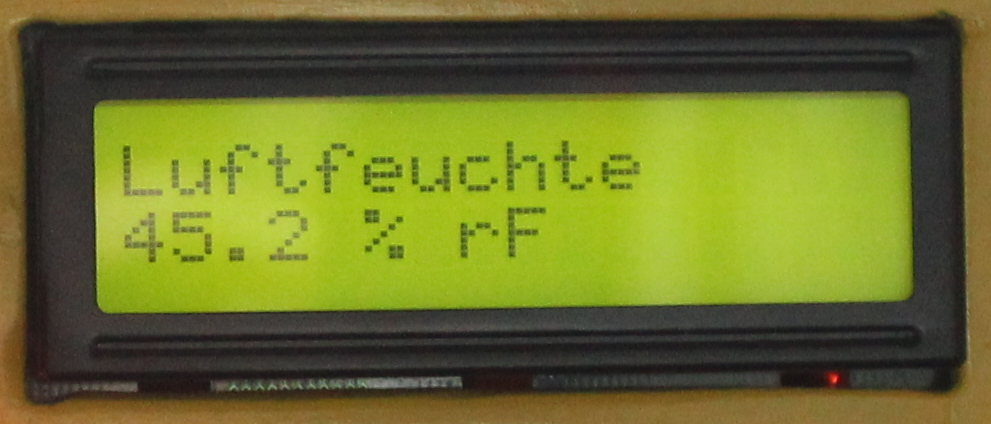
\includegraphics[width=0.9\textwidth]{figures/display.jpg}
  \caption{eingebautes Display (eigenes Werk)}
  \label{fig:display_alt}
\end{figure}

\section{Webinterface}
\label{sec:Webinterface}

Einer der wichtigsten Teile des Projektes ist die grafische Auswertung. Diese kann live auf der Webseite des Raspberry Pi und zeitverzögert unter \href{http://winkler.kremszeile.at}{winkler.kremszeile.at} angesehen werden. Die Auswertung besteht aus zwei von einander unabhängigen Teilen. Zum einen gibt es die Anzeige der Live-Daten, zum anderen die Darstellung der kompletten Aufzeichnung als interaktives Diagramm.

\subsection{Livedaten}
\label{subsec:Livedaten}

\begin{figure}[h]
  \centering
     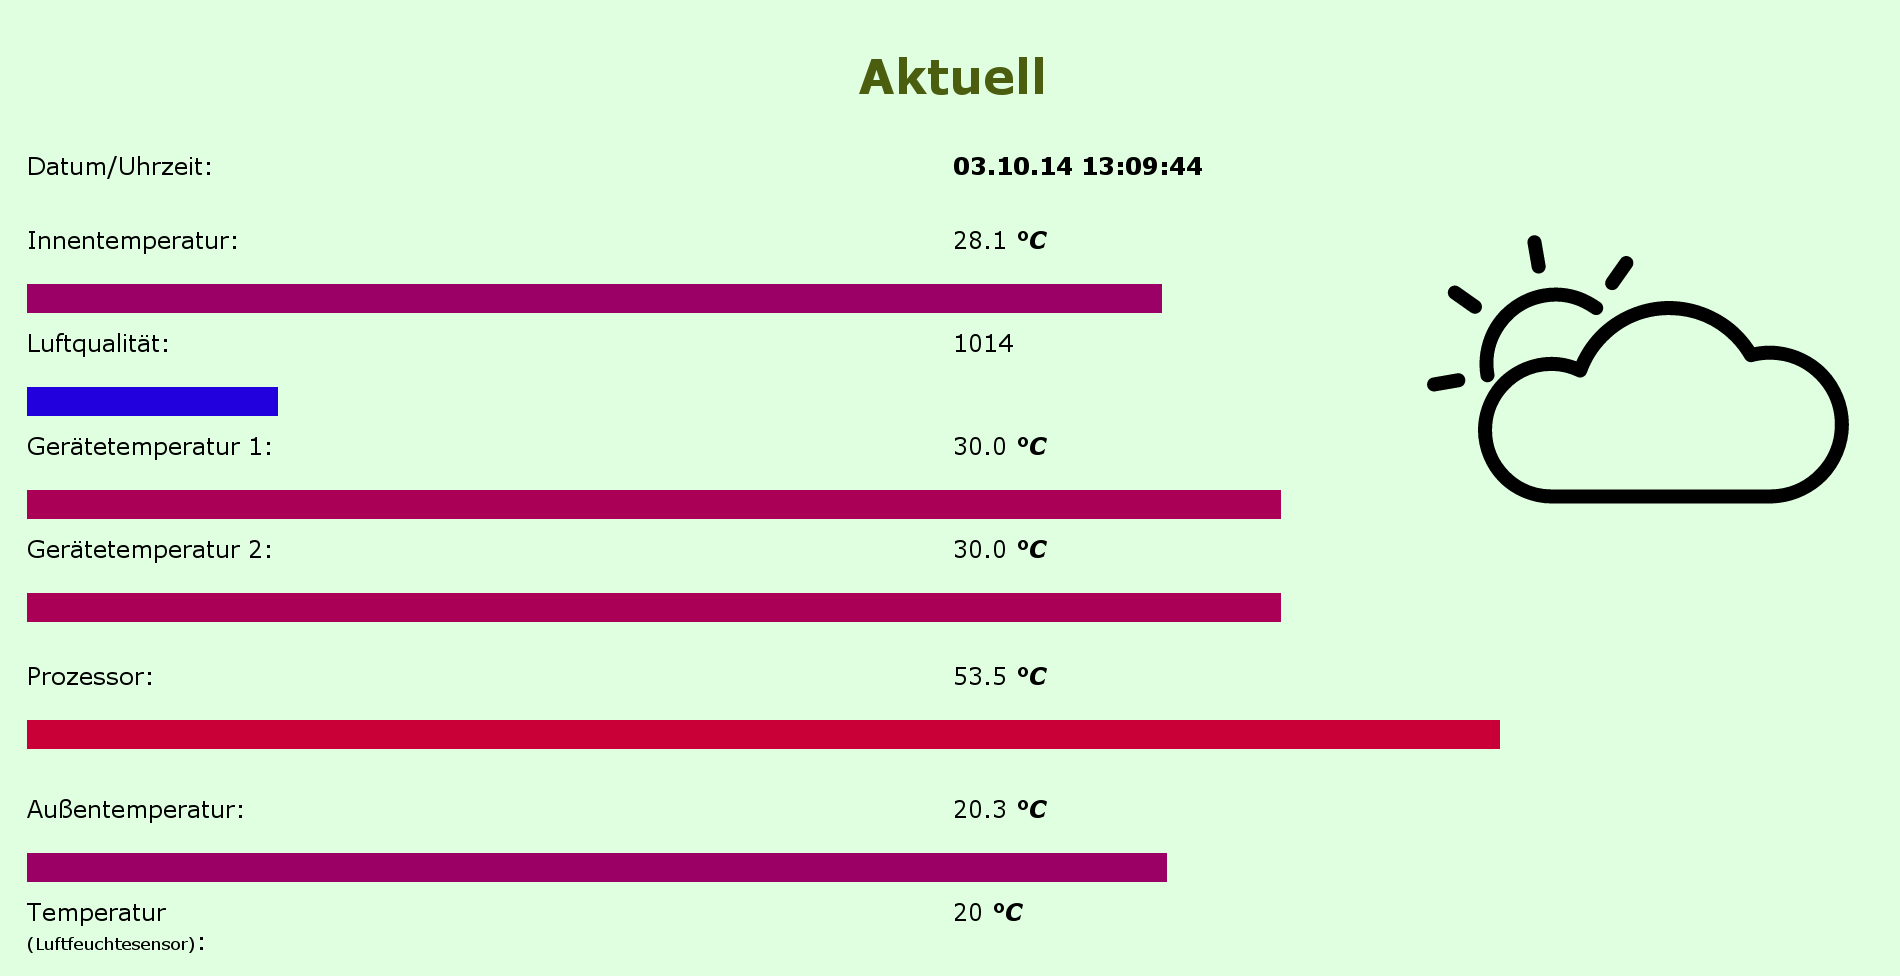
\includegraphics[width=\textwidth]{figures/aktuell.png}
  \caption{Livedaten (eigenes Werk von \href{http://winkler.kremszeile.at/aktuell.html}{winkler.kremszeile.at/aktuell.html})}
  \label{fig:display_neu}
\end{figure}

Auf der Webseite des Raspberry Pi können die aktuellen Messwerte angezeigt und grafisch veranschaulicht werden. Hierzu wird alle 5 Sekunden mithilfe von \gls{Javascript} die Datei \emph{text\_ws.txt} nachgeladen und ausgewertet. Zusätzlich zur Anzeige der Zahlenwerte werden die Messungen mithilfe von Balken und Farbverläufen angezeigt. Zusätzlich gibt es für ältere Browser eine einfache tabellarische Ansicht\footnote{\href{http://winkler.kremszeile.at/aktuell_einfach.html}{winkler.kremszeile.at/aktuell\_einfach.html}}

\subsubsection{Wetterrater}
\label{subsubsec:Wetterrater}

Um die Daten auch anders zu nutzen habe ich einen \emph{Wetterrater} programmiert. Dieser versucht auf Basis von einfachen Berechnungen und Schätzungen das aktuelle Wetter zu \enquote{schätzen}. Es gibt drei Werte aus:
\begin{itemize}
	\item Tag oder Nacht
	\item Niederschlag (keiner/Gewitter/Schnee/Regen/Schneeregen)
	\item Bewölkungsgrad (sonnig/leicht bewölkt/stark bewölkt)
\end{itemize}
Aus diesen Werten wird dann eine Grafik (siehe Abbildung \ref{fig:wettericons}) bestimmt, welche dann angezeigt wird.

\begin{figure}[h]
  \centering
     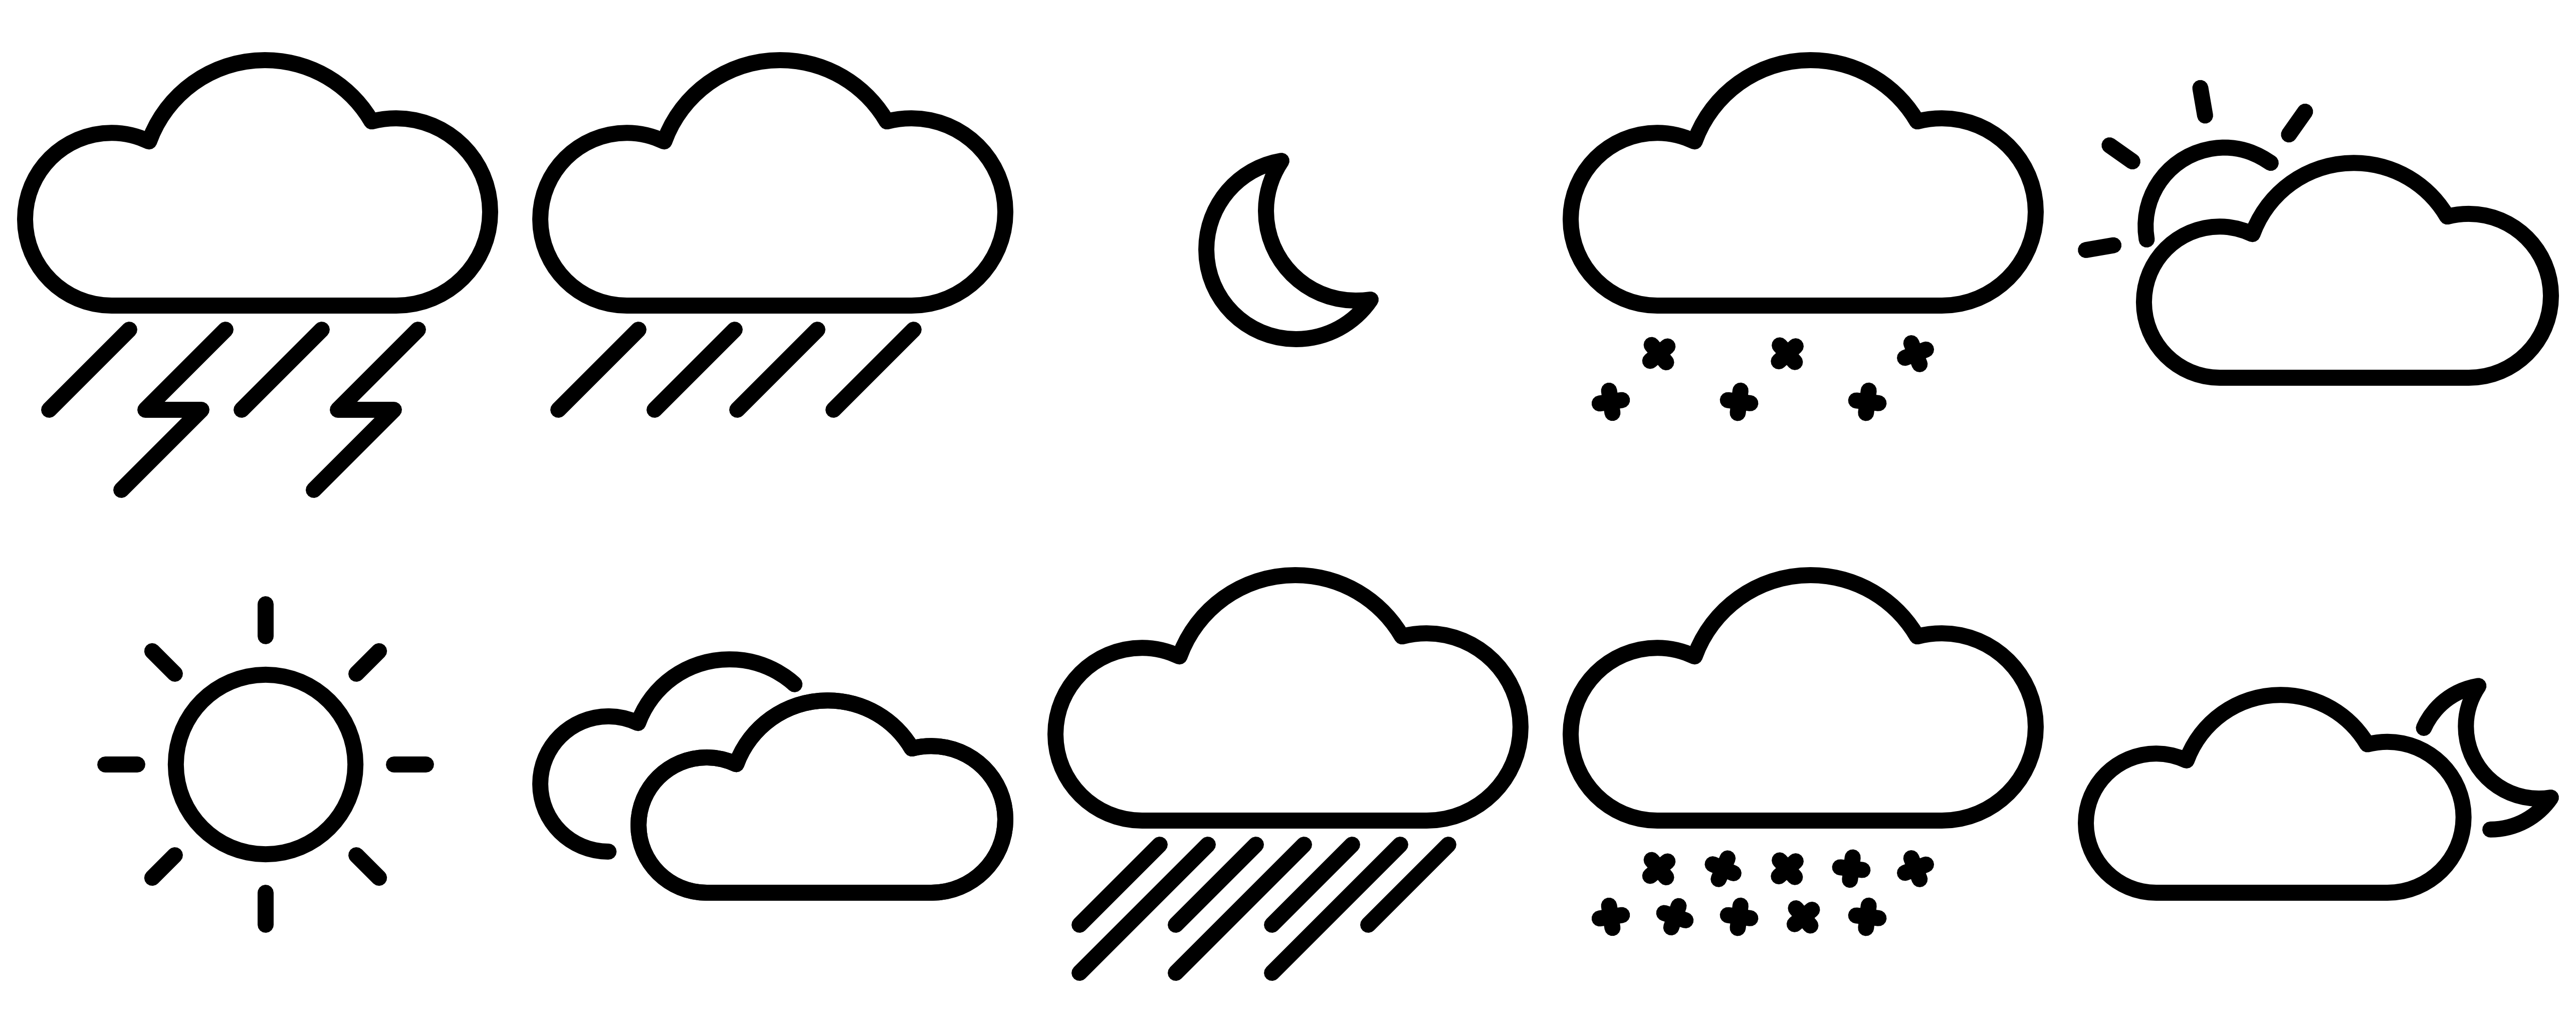
\includegraphics[width=\textwidth]{figures/wettericons.png}
  \caption{Wettericons (eigenes Werk)}
  \label{fig:wettericons}
\end{figure}

\subsection{Diagramme}
\label{subsec:Diagramme}


%%\begin{lstlisting}[language=bash,style=terminal]
%%lukas@kinderzimmer:~$ main.sh -h
%%-d csv-Datei leeren 
%%für weitere Informationen siehe http://winkler.kremszeile.at/ oder https://github.comFindus23/Umweltdatenmessung
%%\end{lstlisting}
